\section{System design} \label{sec:system design}
This section of the report deals with the design of the main parameters of the wind turbine here after called AlphaWind. The parameters are determined for the wind speed distribution encountered in the Western Cape region of South Africa. The wind speed measurements used to determine the Weibull distribution are obtained from a Wind Mast (WM04) near the town of Vredenburg, Western Cape, South Africa seen in Figure \ref{fig:windlocation}.


\subsection{Summary of the design}

The main parameters of the designed wind turbine are presented in Table \ref{tab:systdesign1} and \ref{tab:systdesign2}. Supporting information for calculations can be found in Section 2.2.

\begin{table}[H]
\begin{center} 
\caption{Objectives and boundary conditions}\label{tab:systdesign1}
\begin{tabular}{ |l|c| } 
\hline
\textbf{Parameter} & \textbf{Value/Description}  \\ 
\hline
Onshore or Offshore & Onshore  \\ 
\hline
Type of location & Shrubs \\ 
\hline
Wind conditions: Weibull scale factor & 7.5734 \\
\hline
Wind conditions: Weibull shape factor & 2.1416 \\
\hline
Noise constraint (max tip speed) & 73.6 m/s \\
\hline
Visual constraint & - \\
\hline
\end{tabular}
\end{center}
\end{table}

\begin{table}[H]
\begin{center} 
\caption{Design variables/choices}\label{tab:systdesign2}
\begin{tabular}{ |l|c| } 
\hline
\textbf{Parameter} & \textbf{Value/Description}  \\ 
\hline
Rated power & 2 MW  \\ 
\hline
Number of blades & 3 \\ 
\hline
Rotor diameter & 100.0 m \\
\hline
Design tip speed ratio & 7.67 \\
\hline
Rotational speed range & 7.56 - 14.36 rpm \\
\hline
Cut-in wind speed & 3.04 m/s \\
\hline
Cut-out wind speed & 25.00 m/s \\
\hline
Rated wind speed & 9.85 m/s\\
\hline
Hub height & 70.36 m\\
\hline
\end{tabular}
\end{center}
\end{table}

\subsection{Supporting material, analyses and rationale}

The wind turbine AlphaWind designed and described in this report is made for a location near the town of Vredenburg in Western Cape, South Africa, due to the current interest to increase the energy portfolio through investments in off-grid solutions and renewable sources. The relatively high wind speeds along the coast makes the location a good spot for a wind turbine. The rated power of the wind turbine is set through estimations of a reasonable size of a wind turbine at the established location. For an onshore wind turbine a commonly used size is of a rated power of 2 MW \cite{southafrica}. The number of blades is set to three since turbines with three blades have a slightly higher efficiency than turbines with only two blades and since they are more pleasant for the eye to watch. The reference turbine also have three blades which makes future calculations and comparisons with the reference turbine easier and more accurate. The hub height at this stage is calculated using scaling from the reference turbine.

The turbine is decided to be onshore due to the high cost of an offshore wind turbine project which is currently only feasible with government support. There currently are development projects both onshore and offshore, but according to information retrieved there are no active projects at the chosen location. The maximum tip speed is chosen from noise constraint scaled from the reference turbine for the optimum radius calculated for the new turbine. No visual constraint has been taken in to account since the wind turbine is placed on a field outside of the town of Vredenburg where no activity usually takes place. The calculations for the optimum radius is presented below.

The wind conditions are determined by the parameters of a Weibull distribution for the 10-minute averaged wind speed. This is done by the use of wind data retrieved from the site at a hub height of 62 m, the highest height with available data. These parameters are thereafter used to compute the wind distribution. The wind distribution is used to give the energy yield as a function of the theoretical power curve according to Equation \ref{eq:E}. The power curve is computed according to Equation \ref{eq:P} as a function of the radius. The radius is varied from $30 m$ to $120 m$. The equations for energy yield and the power curve are thereafter solved simultaneously to find the variation of the energy yield for different values of the radius. To determine the optimal radius, the normalised cost over energy yield has been computed, assuming that the normalised total cost for onshore wind turbines can be calculated using Equation \ref{eq:C}.


\begin{equation}
E_{y}\ = \sum_{i} P_{i}\, h_{i}\, \Delta \, v
\label{eq:E}
\end{equation}

\begin{equation}
P = \frac{\pi\, \mathrm{Cp}\, R^2\, \rho\, v^3}{2}
\label{eq:P}
\end{equation}

\begin{equation}
C_{norm}\ = 0.7 + 0.3 {\left(\frac{D}{D_{ref}}\right)}^{2.6}
\label{eq:C}
\end{equation}


\vspace{3mm}

The result of the optimisation is shown in Figure \ref{fig:pcurve} and \ref{fig:costey}.

\begin{figure}[H]
\centering
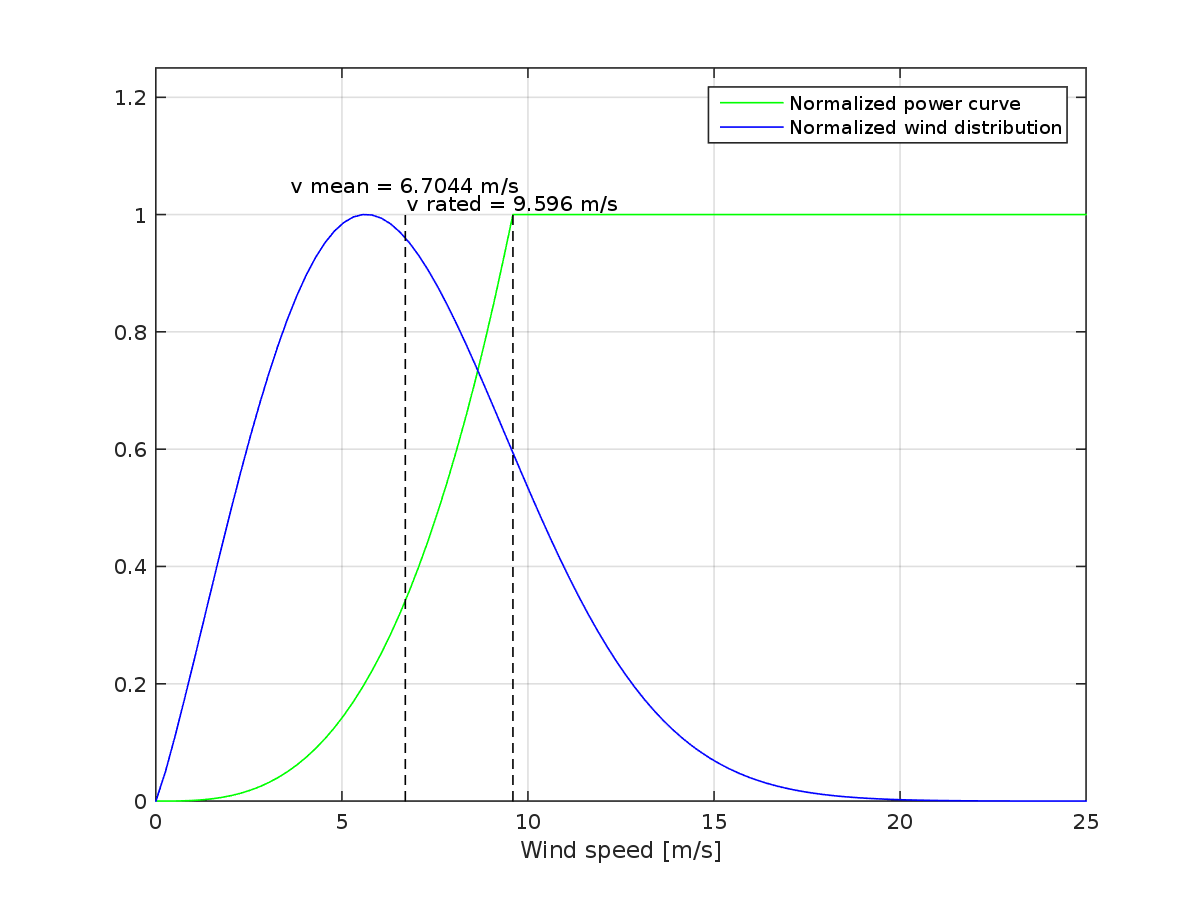
\includegraphics[width=0.7\textwidth]{Images/power_curve.png} 
\caption{Normalised power curve and wind distribution}\label{fig:pcurve}
\end{figure}

\begin{figure}[H]
\centering
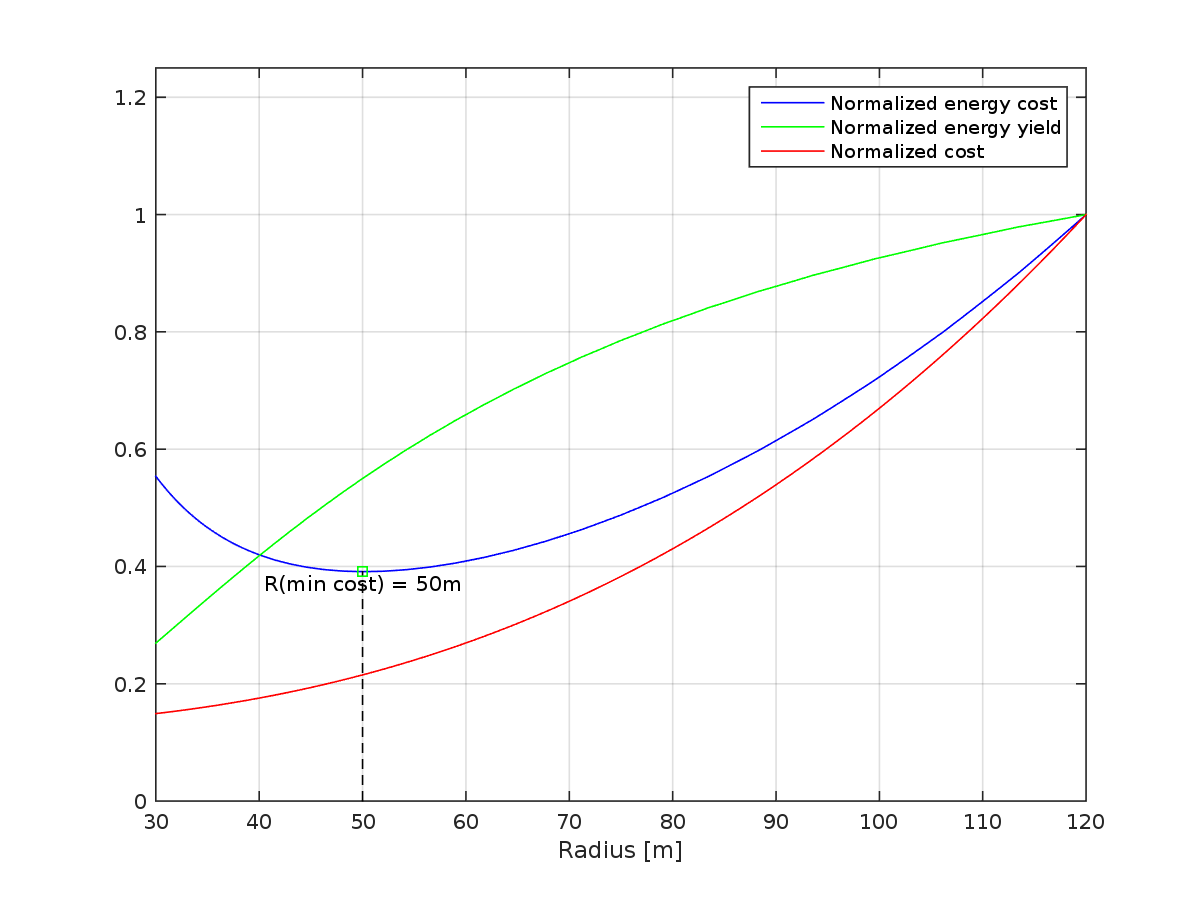
\includegraphics[width=0.7\textwidth]{Images/optimal_cost.png} 
\caption{Normalised energy cost as a function of radius}\label{fig:costey}
\end{figure}

Figure \ref{fig:pcurve} shows the normalised power curve and the normalised wind distribution as a function of the wind speed. The rated wind speed is 9.8 m/s while the mean wind speed at he location is 6.7 m/s. Figure \ref{fig:costey} shows the normalised cost (red line) and the normalised energy yield (green line) as well as the normalised cost over energy yield (blue line), all as a function of the rotor radius. The later shows a minimum at a radius of 50.0 m. At this radius the turbine will produced the highest energy yield at the lowest cost which makes it the optimum radius for the designed wind turbine. The optimum rotor diameter is therefore set to 100.0 m.

The normalised curves in Figure \ref{fig:costey} have been calculated as follows. The cost over energy yield is calculated for each rotor radius and thereafter divided by the maximum value of the cost over energy yield. The same method is used for the remaining two curves, the energy yield is calculated for each rotor radius and thereafter divided by the maximum value of the energy yield, and the cost is calculated for each rotor radius and thereafter divided by the maximum value of the cost.